\section{Shared Space}
\label{sec:shared_space}
Dette afsnit er inspireret af siden Vejdirektoratet. \autocite{vejlednigomss2013} \\
Shared space er et begreb, der definerer en vejledning til trafik- og byplanlæggere. Vejledningen giver anbefalinger til vejmyndigheder, rådgivere og arkitekter der fortæller noget om, hvordan shared space burde anvendes, skiltes og udformes, som en indretning af gaderum i de danske byer. Derudover indeholder vejledningen anbefalinger til, hvilke trafikmængder og hastigheder der bør være i et shared space område.

\subsubsection{Fremføring til Shared Space}
\label{subs:fremforing_til_shared_space}

Shared space konceptet udkom i forbindelse med, at den hollandske trafik ingeniør Hans Monderman blev kendt i medierne for sin løsning til, hvordan trafiksikkerheden kunne øges, ved at der skulle mindskes vejskilte og trafiklys. Tanken er at trafikområdet bliver reguleret i bekendtskab med trafikantgruppernes sunde fornuft, idet at de deles om området. Det resulterede i at en række EU lande samarbejdede om shared space konceptet, der også havde til formål at udvikle nye rumlige designkoncepter, hvor der skulle være plads til trafik og ophold. \autocite{DEFT2006}
\\
Shared space indebærer, at de forskellige trafikantgrupper så som den kollektive trafik, privatbiler, parkering, godstrafik, cykelister og fodgængere deler det offentlige rum med hinanden, uden at nogle grupper burde være dominerende. Shared space konceptet er for det offentlige byrum en prioritering af det sociale liv for mennesker. Derudover stræber det efter at skabe velfungerende og multifunktionelle byrum, hvor alle trafikantgrupper er ligeværdige i trafikken. Alle trafikantgrupper integreres og færdes på samme areal. Shared space’s fysiske udformning er et område, hvor der ikke er nogle traditionel opdeling for fodgængere, cyklister og kørertøjer. Her er der et minimum af skiltninger og afmærkninger.
\\\\
\subsubsection{Historisk tilbageblik på Shared Space}
\label{subs:historisk_tilbageblik_paa_shared_space}
Der var et fredeligt samspil mellem trafikantgrupperne, hvor byrummene typisk fungerede som shared space, indtil massebilismen indtog, hvor man herefter begyndte med at differentiere trafikantgrupperne for at modvirke uheldene. Den hurtige trafik skulle skilles fra den langsomme, og den hårde trafik fra den bløde. Der blev etableret separate cykel- og gangstier på de større veje. Grundidéen blev udviklet med specielt henblik på de mange nye byområder og var et udtryk for ønsket om, at sikre både biltrafikkens sikkerhed og skabe trafiksikre boligområder. Der blev etableret en lang række trafikdifferentierede byområder både i Danmark og udlandet i perioden 1960-1975.
\\
I begyndelsen af 1970’erne blev integrationen mellem de bløde og hårde trafikanter første gang genintroduceret i Holland, som en modreaktion på differentiering af trafikanterne i byområderne. På derværende tidspunkt blev der i hollandske boligområder etableret ”woonerven” (bebolig gader). Ønsket var grundlæggende at reducere antallet af kørende og deres hastighed. Det foregik gennem etablering af fysiske ændringer såsom bump, forsætninger og indsnævringer af kørebanearealet, samt ved bevidst brug af beplantning og pynte området. Formålet med de fysiske ændringer var for, at lade bilerne køre i gaderne, men med meget lave hastigheder, for at tage hensyn til fodgænger og legende børns betingelser.  Det resulterede en lang række kopieringer og fortolkninger af de hollandske initiativer, især i Nordeuropa eksempelvis i Home Zone i Storbritannien, Spielstrassen i Tyskland, gårdsgader i Danmark og Sverige i opholds- og legeområder.
Byer med gader og torve har altid indeholdt flere funktioner.  Byrummene har blandt andet den funktion, at den burde kunne afvikle trafikken bestående af kollektiv trafik, privatbiler, parkering, godstrafik, cykelister og fodgængere. Derudover har byrummene også til funktion, at blive brugt til ophold og handel for byens beboere og besøgende.
Integration af både forskellige trafikantgrupper og opholdsfunktioner kan opleves nogle steder i vores byer og andre steder i Nordeuropa. Denne trafikalblanding har gennem tiderne blevet kaldt mange forskellige ting. Siden starten af 1980’erne er der især i Nordeuropa blevet udformet en lang række forskellige nye blandede trafik- og opholdsrum. \autocite{vejlednigomss2013}Hvilket blandt andet kan ses i den Østrigske by Ganz i Sonnenfelsplatz, som er et shared space område, hvor trafikantgrupperne indretter sig efter hinandens adfærd.\autocite{SP2015}

\subsubsection{Andre type gader}
\label{subs:andre_type_gader}

%\label{sec:Andre type gader}
Der findes andre type gader som også kan minde om shared space. Disse type gader har andre tilgange til, hvor og hvordan området bliver udformet. Derudover prioritere de trafikantgruppernes ophold anderledes end shared space.

\subsubsection{Gågader}
\label{subs:gaagader}

I begyndelsen af 1960’erne blev en række tideligere gader ændret til gågader. Det typiske ved gågader er, at de ofte ligger centralt ved beliggende butiks- eller strøggader, som primært er indrettet til gående, hvor biltrafik er fjernet med undtagelse af varekørsel. Derfor er gågader kendetegnet ved, at være trafikale differentierede gadetyper.
Gågaders karakteristiske fysiske udformning er en indretning, hvor belægningen fremtræder forskelligt fra traditionelle kørearealer. For at få gågaden til at fremstå sammenhængende fra facade til facade, bliver niveauforskellene mellem fortov og vej fjernet. I andre sammenhænge etableres gågader, hvor kørselstilladelse, som er eksisterende for den bevidste udformede sivegade. \autocite{vejlednigomss2013} %\autocite{}
\begin{figure}[htbp]
  \centering
  \begin{adjustbox}{max width=\textwidth}
    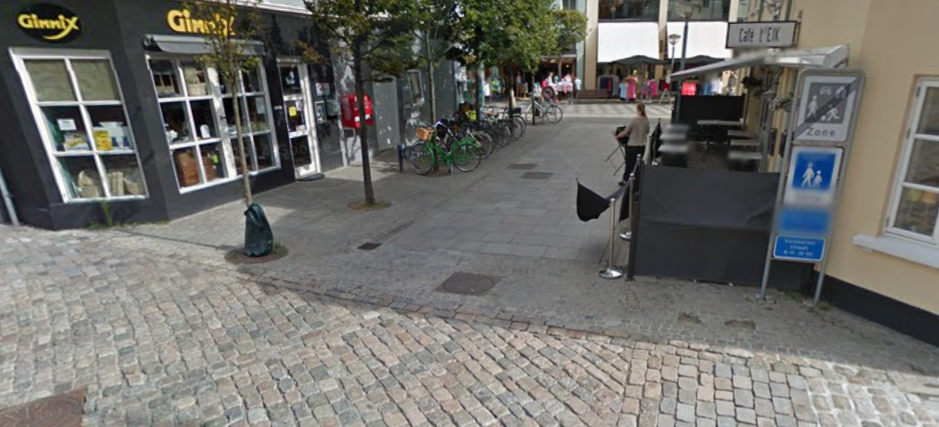
\includegraphics{figures/Billederogfigur/Indledningen/gaagade_ved_slotsgade.png}
 \end{adjustbox}
  \caption{Niveauforskel på belægning og gågade skilt i Søndergade, Aalborg \autocite{gm2015}}
    \label{fig:nivbelaegningegaagade}
\end{figure}

\subsubsection{Sivegader}
\label{subs:sivegader}

I midten af 1980’erne begyndte man med, at ombygge mere centrale beliggende by-gader og handelsstrøg med større trafikmængder til sivegaderne, som er nogle stilleveje der ikke er defineret som et begreb i færdselsloven. Det karakteristiske ved sivegader er, at de er opbygget med smalle kørebaner uden niveauforskelle til de bagvedliggende arealer, og gaden fremstår oftest som en sammenhængende flade, med markeringer af parkerings- eller udstillings-/opholdsarealer. Helhedsvurderingen er en multifunktionel by-gade og ikke en trafikvej, som er understreget i den fysiske anvendelse af belægninger og belysning, det kendetegnes fra gågader, som i højere grad er afgørende for opfattelsen af byrummets karakter og den ønskede trafikale facon. I sivegader er der oftest skiltet med C55 lokal hastighedsbegrænsninger til 20 km/t eller 30 km/t, som ses på figur \cref{fig:lokalhastighedfart} side \pageref{fig:lokalhastighedfart}, og E53 områder med fartdæmpning, som fortæller at området ikke er egnet til kørsel med højere hastigheder end den er angivet til\autocite{hs}


eller med andre tilfælde E49 gågade med kørsel tiltalt som undertavle, som ses på figur \cref{fig:fartdaempning} side \pageref{fig:fartdaempning} og på figur \cref{fig:gaagadeskilt} side \pageref{fig:gaagadeskilt}.\autocite{vejlednigomss2013}

\begin{figure}[htbp]
  \centering
  \begin{adjustbox}{max width=\textwidth}
    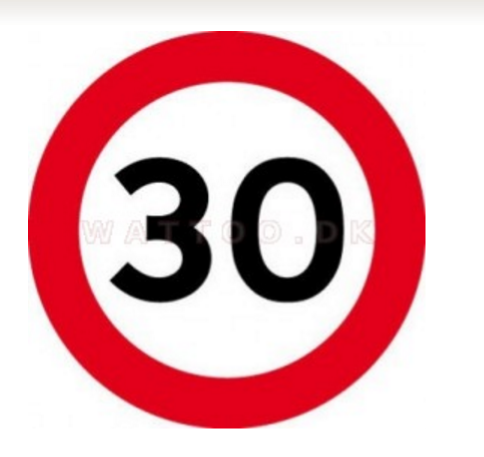
\includegraphics[scale=0.3]{figures/Billederogfigur/Indledningen/lokal_hastighedsberaensning_c55_30km.png}
 \end{adjustbox}
  \caption{C55 Lokalhastighedsbegrænsning \autocite{forbudsskilt2007}}
    \label{fig:lokalhastighedfart}
\end{figure}

\begin{figure}[htbp]
  \centering
  \begin{adjustbox}{max width=\textwidth}
    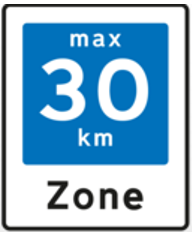
\includegraphics[scale=0.5]{figures/Billederogfigur/Indledningen/E53.png}
 \end{adjustbox}
  \caption{E53 Fartdæmpning skilt \autocite{e49}}
    \label{fig:fartdaempning}
\end{figure}

\begin{figure}[htbp]
  \centering
  \begin{adjustbox}{max width=\textwidth}
    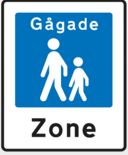
\includegraphics{figures/Billederogfigur/Indledningen/E49.png}
 \end{adjustbox}
  \caption{E49 Gågade skilt \autocite{e49}}
    \label{fig:gaagadeskilt}
\end{figure}



\subsubsection{Andre typer gader sammenlignet med shared space}
\label{subs:andre_typer_gader_sammenlignet_med_shared_space}

Sivegader og andre forskellige gadetyper kan på mange måder ses som shared space- ligende gaderum, men alligevel adskiller de sig fra shared space. Shared space anvendes primært i centrale byområder, hvor der er høj trafikmængder, her er hensigten at trafikantgrupperne skal kunne færdes under fælles hensyntagen, hvorimod at andre gadetyper anvendes i primært boligområder med meget lav trafikmængder, hvor hensigten er at skabe mulighed for leg og ophold i vejens bredde.
Fælles for gågader og shared space områder er at de begge er beliggende i centrale byområder. Forskellen mellem gågader og shared space er mængden af trafikanterne i områderne. I gågader er mængden af kørende trafikanter mindre end i shared space, hvor kørsel er tilladt. Kørende trafik færdes under de gåendes betingelser, det vil sige, at de gående er i overtal og prioriteret frem for kørende trafik, da det er en gade for gående. I shared space områder er mængden kørende trafikanter højere end i gågader, her er ingen trafikantgrupper prioriteret frem for andre.
Sivegader minder allermest om shared space områder, da der er en multifunktionel indretning, som ligger til grund for strukturen og udformningen, hvor de forskellige trafikantgrupper færdes ligeværdigt i hele områdets udtrækning og uden den traditionelle fysiske opdeling i gang/opholds- og kørearealer. Skiltning af sivegader er ikke tydelige, da begrebet ikke findes som begreb i færdselsloven, derfor skiltes den forskelligt fra sted til sted.\autocite{vejlednigomss2013}
